This is the week 1 of the course Probabilistic Graphical Models (pgm) by Prof. Daphne Koller hosted on Coursera. The week 1 covers quite a lot of notions from distribution to Bayesian Network.

\section{Distribution}
A probability distribution function (aka PDF, probability density function, probability function, or density) is a function that indicates the probability that a given random variable will take on a particular value. If a random variable is discrete (i.e. the value of the random variable is contained in a countable set of values), then the probability density function, $f(x)$ of a random variable $X$ is: $f(x) = P(X = x)$.

The multivariate form of a probability distribution function is the probability that a list of random variables will take on a list of values. If the random variables are discrete, the \textbf{joint probability density function}, $f(x_1, x_2, …, x_n)$ for random variables $X_1, X_2, ..., X_n$ is defined by: 
\begin{align}
f(x_1, x_2, \ldots, x_n) = P(X_1=x_1, X_2=x_2, \ldots, X_n=x_n)
\end{align}
\myaligns{Joint Distribution}

\section{Conditioning}
It's when we condition on some variables. The data obtained after conditioning is called unnormalized measures and we can make them normalized by divide each of them by their sum. For example, we have a joint distribution $P(I, D, G)$ and we condition on variable $G$ to take only its value $G = g_1$. So we need to delete all measures having $G \neq g_1$. This step is called \textbf{reduction} in conditioning. After this step, we obtain measures that does not sum to 1. So we need to sum them up and divide each measure to this sum in order to obtain a (conditional) probability. This step is called \textbf{renormalization} in conditioning.  

\begin{align}
P(I, D, G) \xrightarrow{reduction} P(I, D, G=g_1) \xrightarrow{renormalize} P(I, D, g_1)
\end{align}
\myaligns{Conditioning}

\section{Marginalization}
It's when we have a large data set and we want to observe it only in terms of some variables. For example we have a joint distribution $P(I, D)$ and we are interested only in variable $D$. So we \textbf{marginalize} $I$ by summing over $I$ for each value that $D$ takes: 
\begin{align}
P(D) = \sum_{I} P(I, D)
\end{align}
\myaligns{Marginalization}


\section{Factors}
A factor is a function or a table or a mapping from every assignment of arguments to a real value. We define below factor $\Phi(X_1, \ldots, X_k)$ where $(X_1, \ldots, X_k)$ which is the scope (a set of random variables).
\begin{align}
\Phi: Val(X_1, \ldots, X_k) \rightarrow \mathbb{R}
\end{align}
\myaligns{Factor Definition}

\subsection{Examples of Factor}
Hence, according to the definition above, a joint distribution is a factor. Figure \ref{w1JointDistri} illustrates a joint distribution $P(I,D,G)$ where $I$, $D$, $G$ represents intelligence of a student $(0, 1)$, difficulty of a course $(0,1)$, and the final grade $(A,B,C)$ that student got from that course respectively.
\begin{figure}[!ht]
\centering
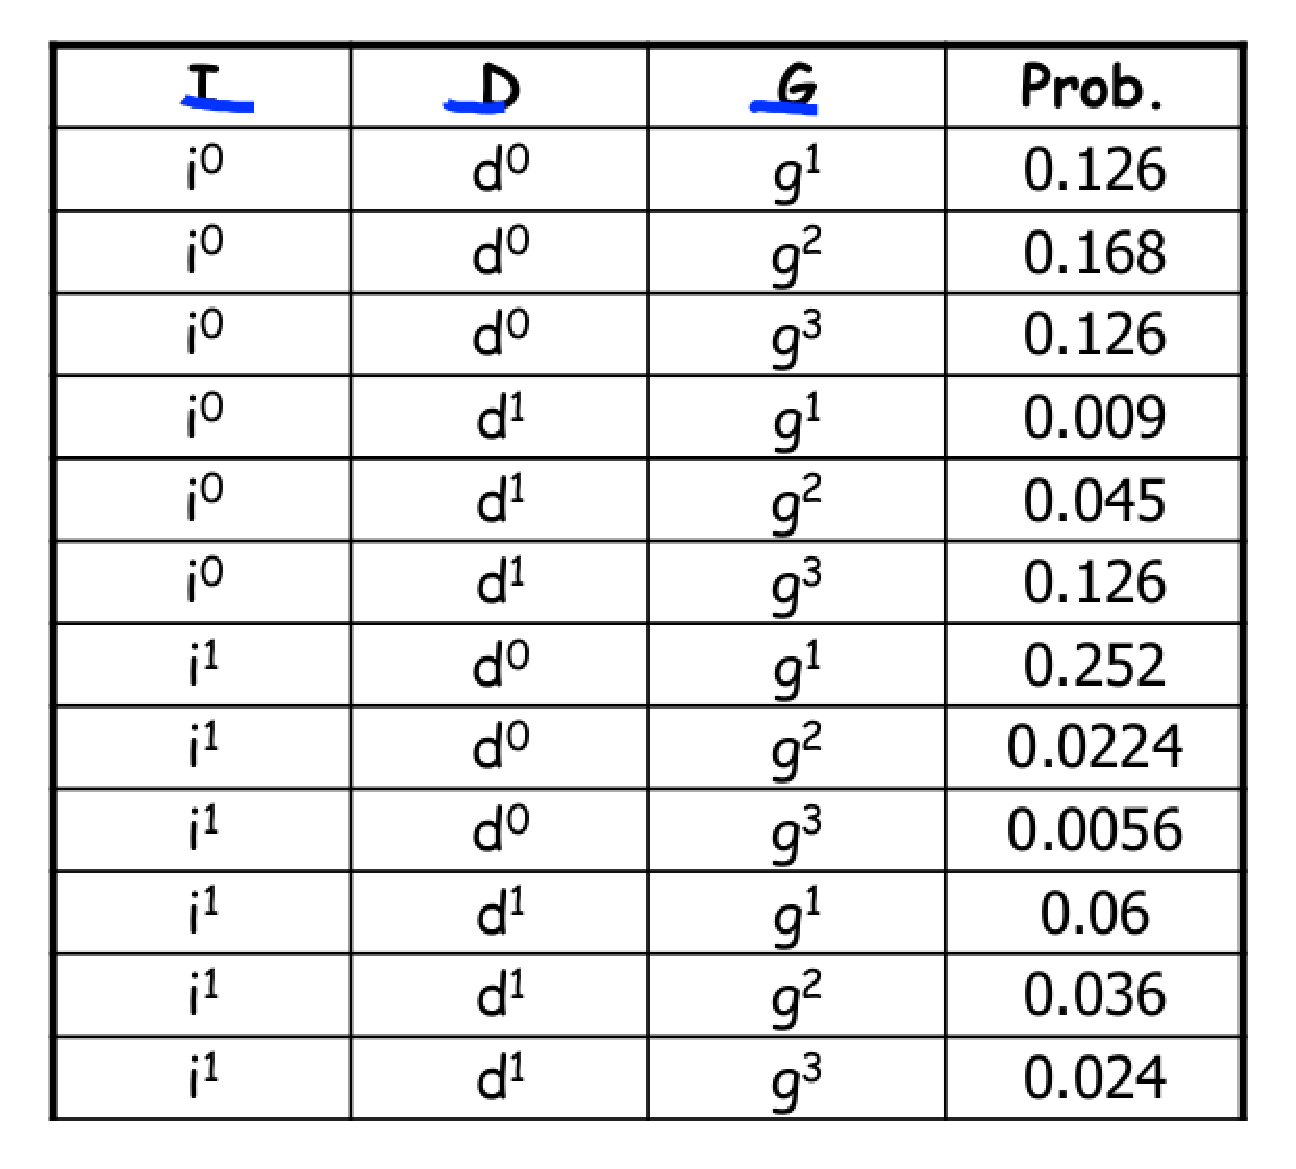
\includegraphics[scale = 0.3]{w1JointDistri}
\caption{Joint Distribution}
\label{w1JointDistri}
\end{figure}

Another example is Unnormalized Measure $P(I,D,g^1)$ which has scope $(I,D)$ because $G$ is always fixed to $g^1$. Another \textbf{important example} is Conditional Probability Distribution (CPD). Figure \ref{w1CPD} illustrates the \textbf{CPD} $P(G | I, D)$ which means for every combination of values to the variable $I$ and $D$, we have a probability distribution over $G$.  

\begin{figure}[!ht]
\centering
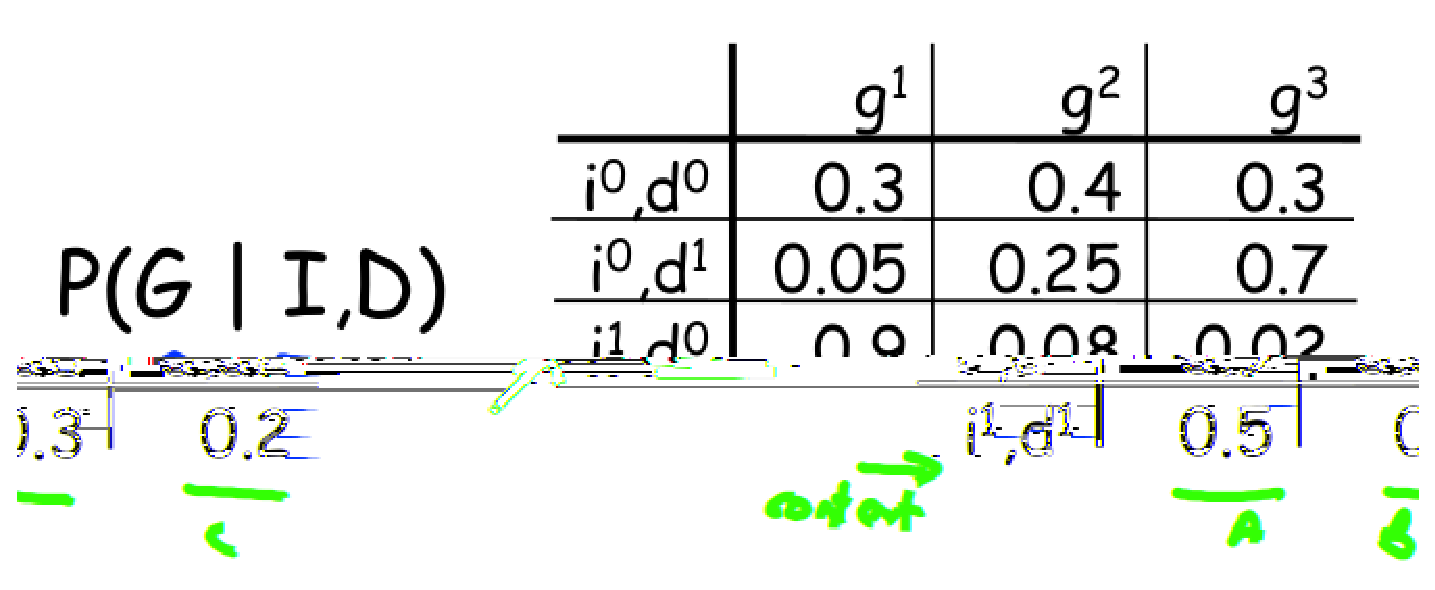
\includegraphics[scale = 0.4]{w1CPD}
\caption{Conditional Probability Distribution (CPD)}
\label{w1CPD}
\end{figure}

\section{Operations on Factors}
\subsection{Factor Products}
If $\Phi_1(A,B)$ and $\Phi_2(B,C)$ are two factors then we compute their product of $\Phi(A,B,C)$ by multiplying $\Phi_1(A,B)\Phi_2(B,C)$ for all common values of $B$ (see figure \ref{w1FactProd}).

\begin{figure}[!ht]
\centering
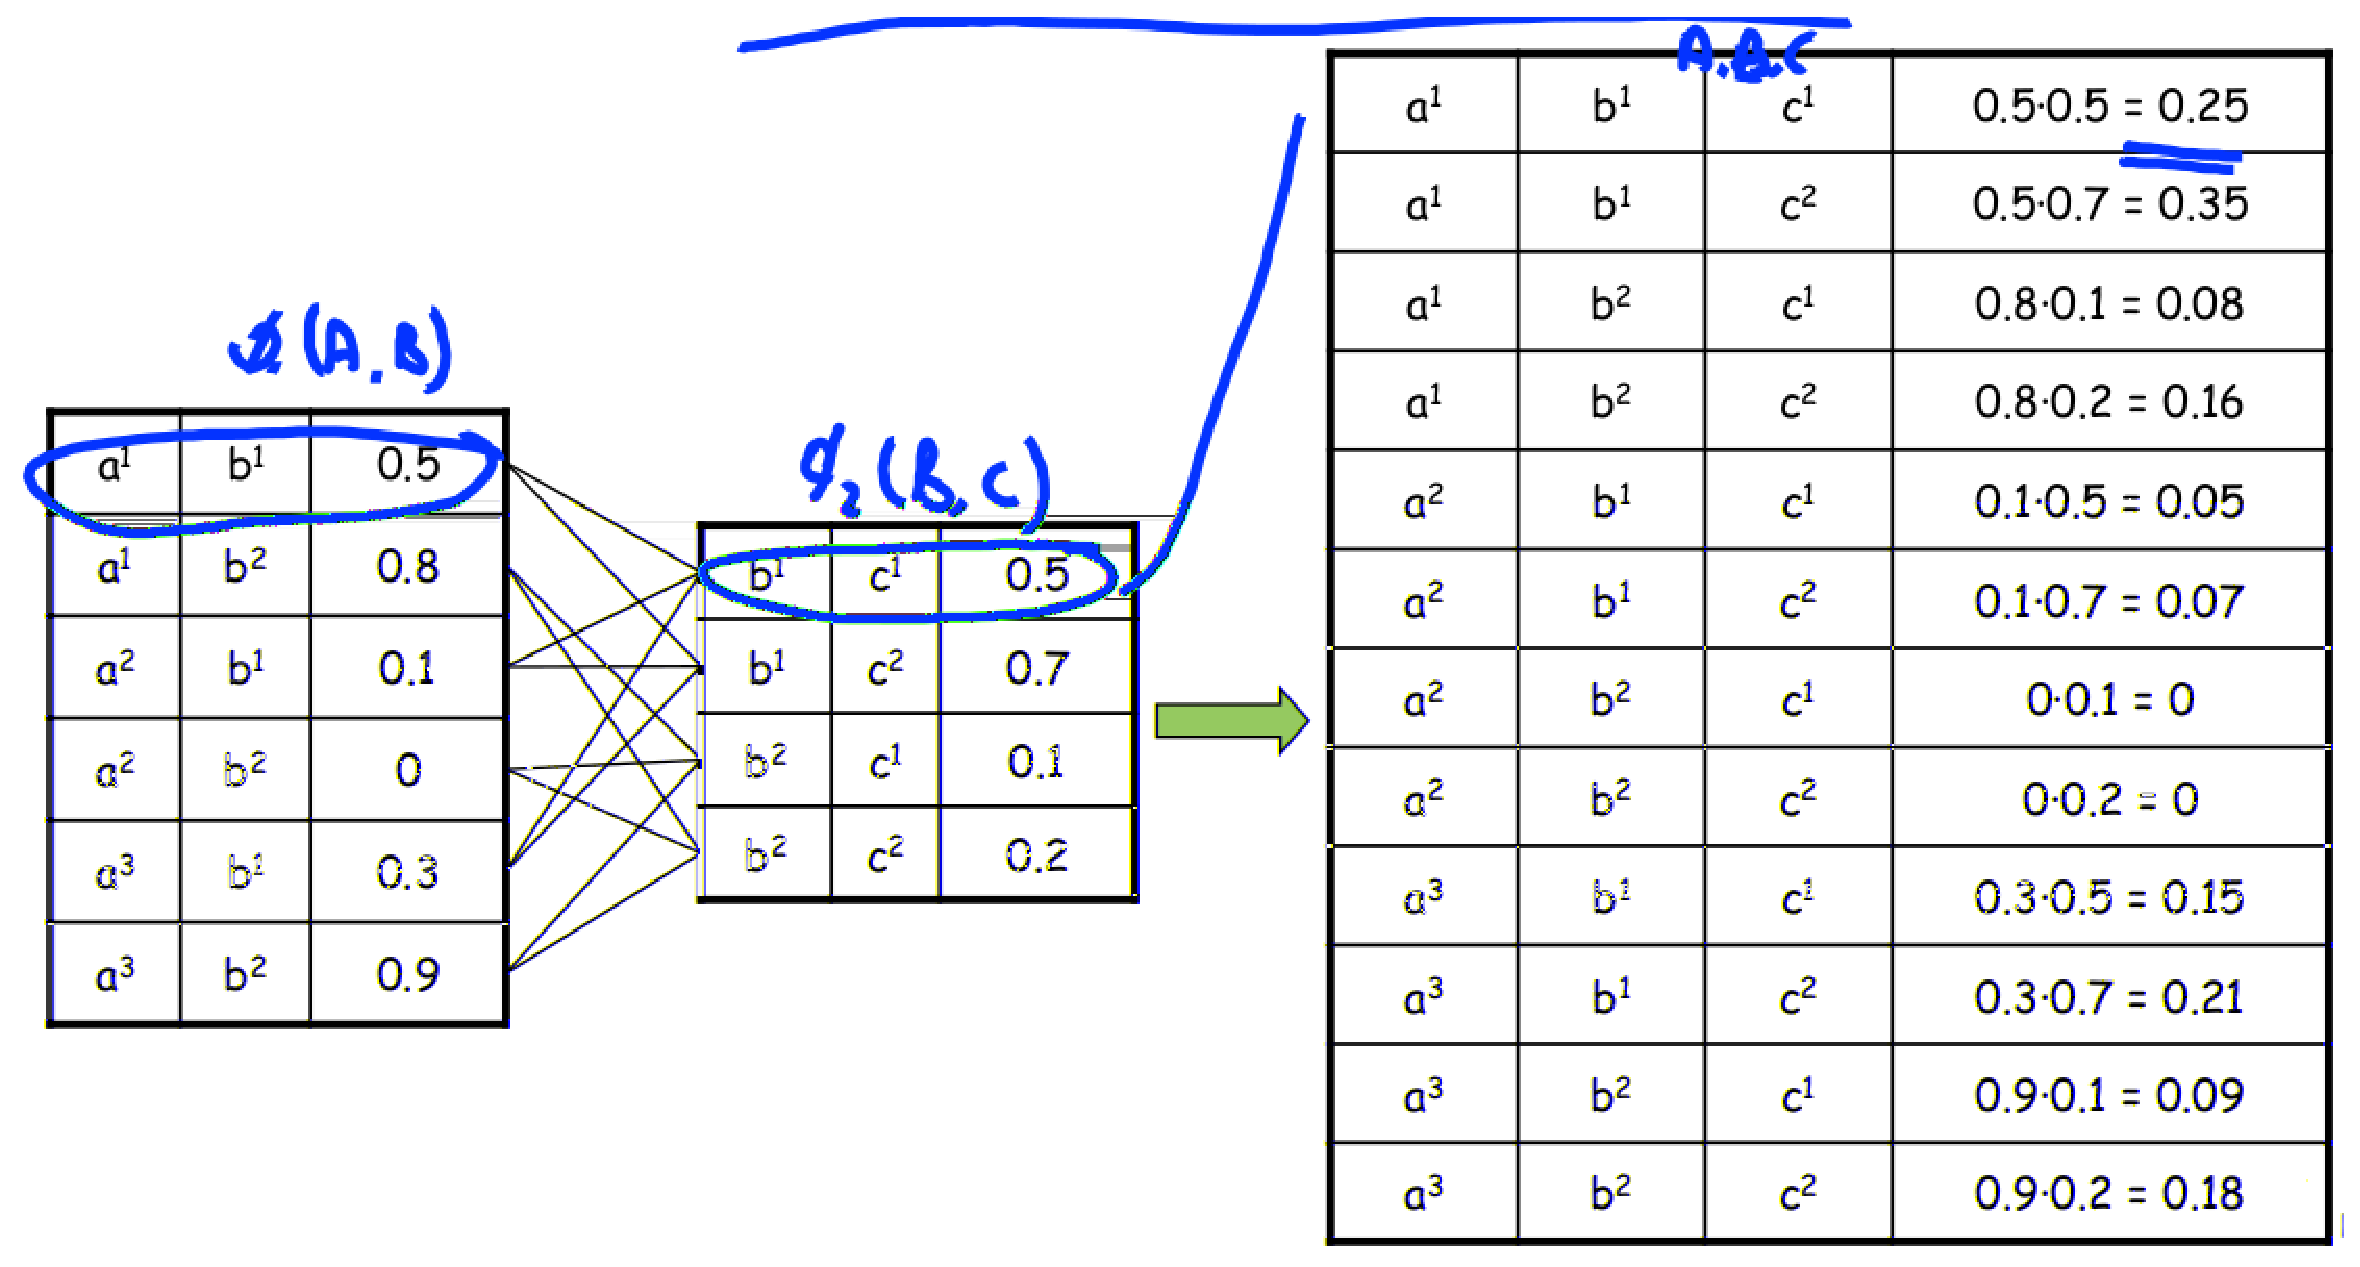
\includegraphics[scale = 0.3]{w1FactProd}
\caption{Factor Products}
\label{w1FactProd}
\end{figure}

\subsection{Factor Marginalization}
That's when we want to reduce the scope. For example, we reduce scope $(A,B,C)$ to $(A,C)$ by summing over $B$ for every assignment of $(A,C)$ (figure \ref{w1FactMarginal}).

\begin{figure}[!ht]
\centering
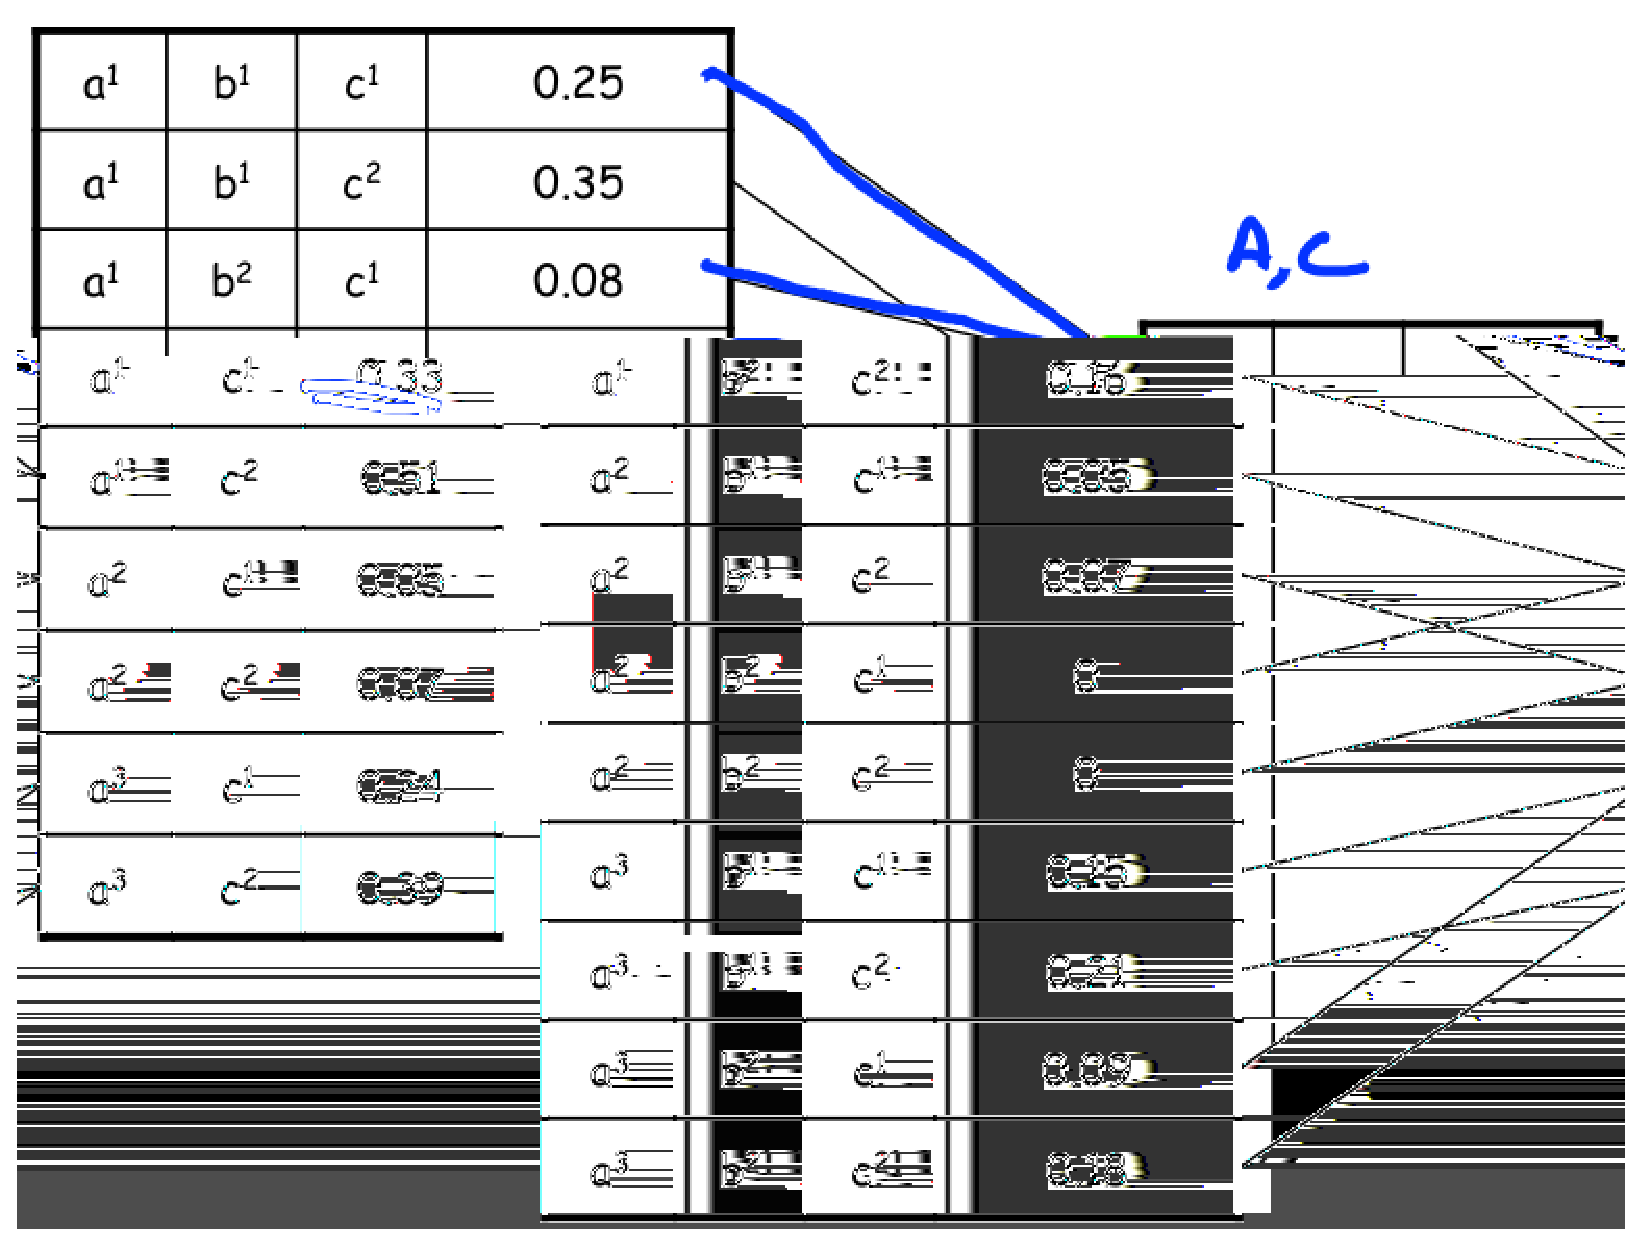
\includegraphics[scale = 0.35]{w1FactMarginal}
\caption{Factor Marginalization}
\label{w1FactMarginal}
\end{figure}

\subsection{Factor Reduction}
That's when we fix a random variable in the scope by one value (in its set of values). For example, $\Phi(A,B,C)$ is reduced to $\Phi(A,B | C = c^1)$ in illustration \ref{w1FactReduce}.
\begin{figure}[!ht]
\centering
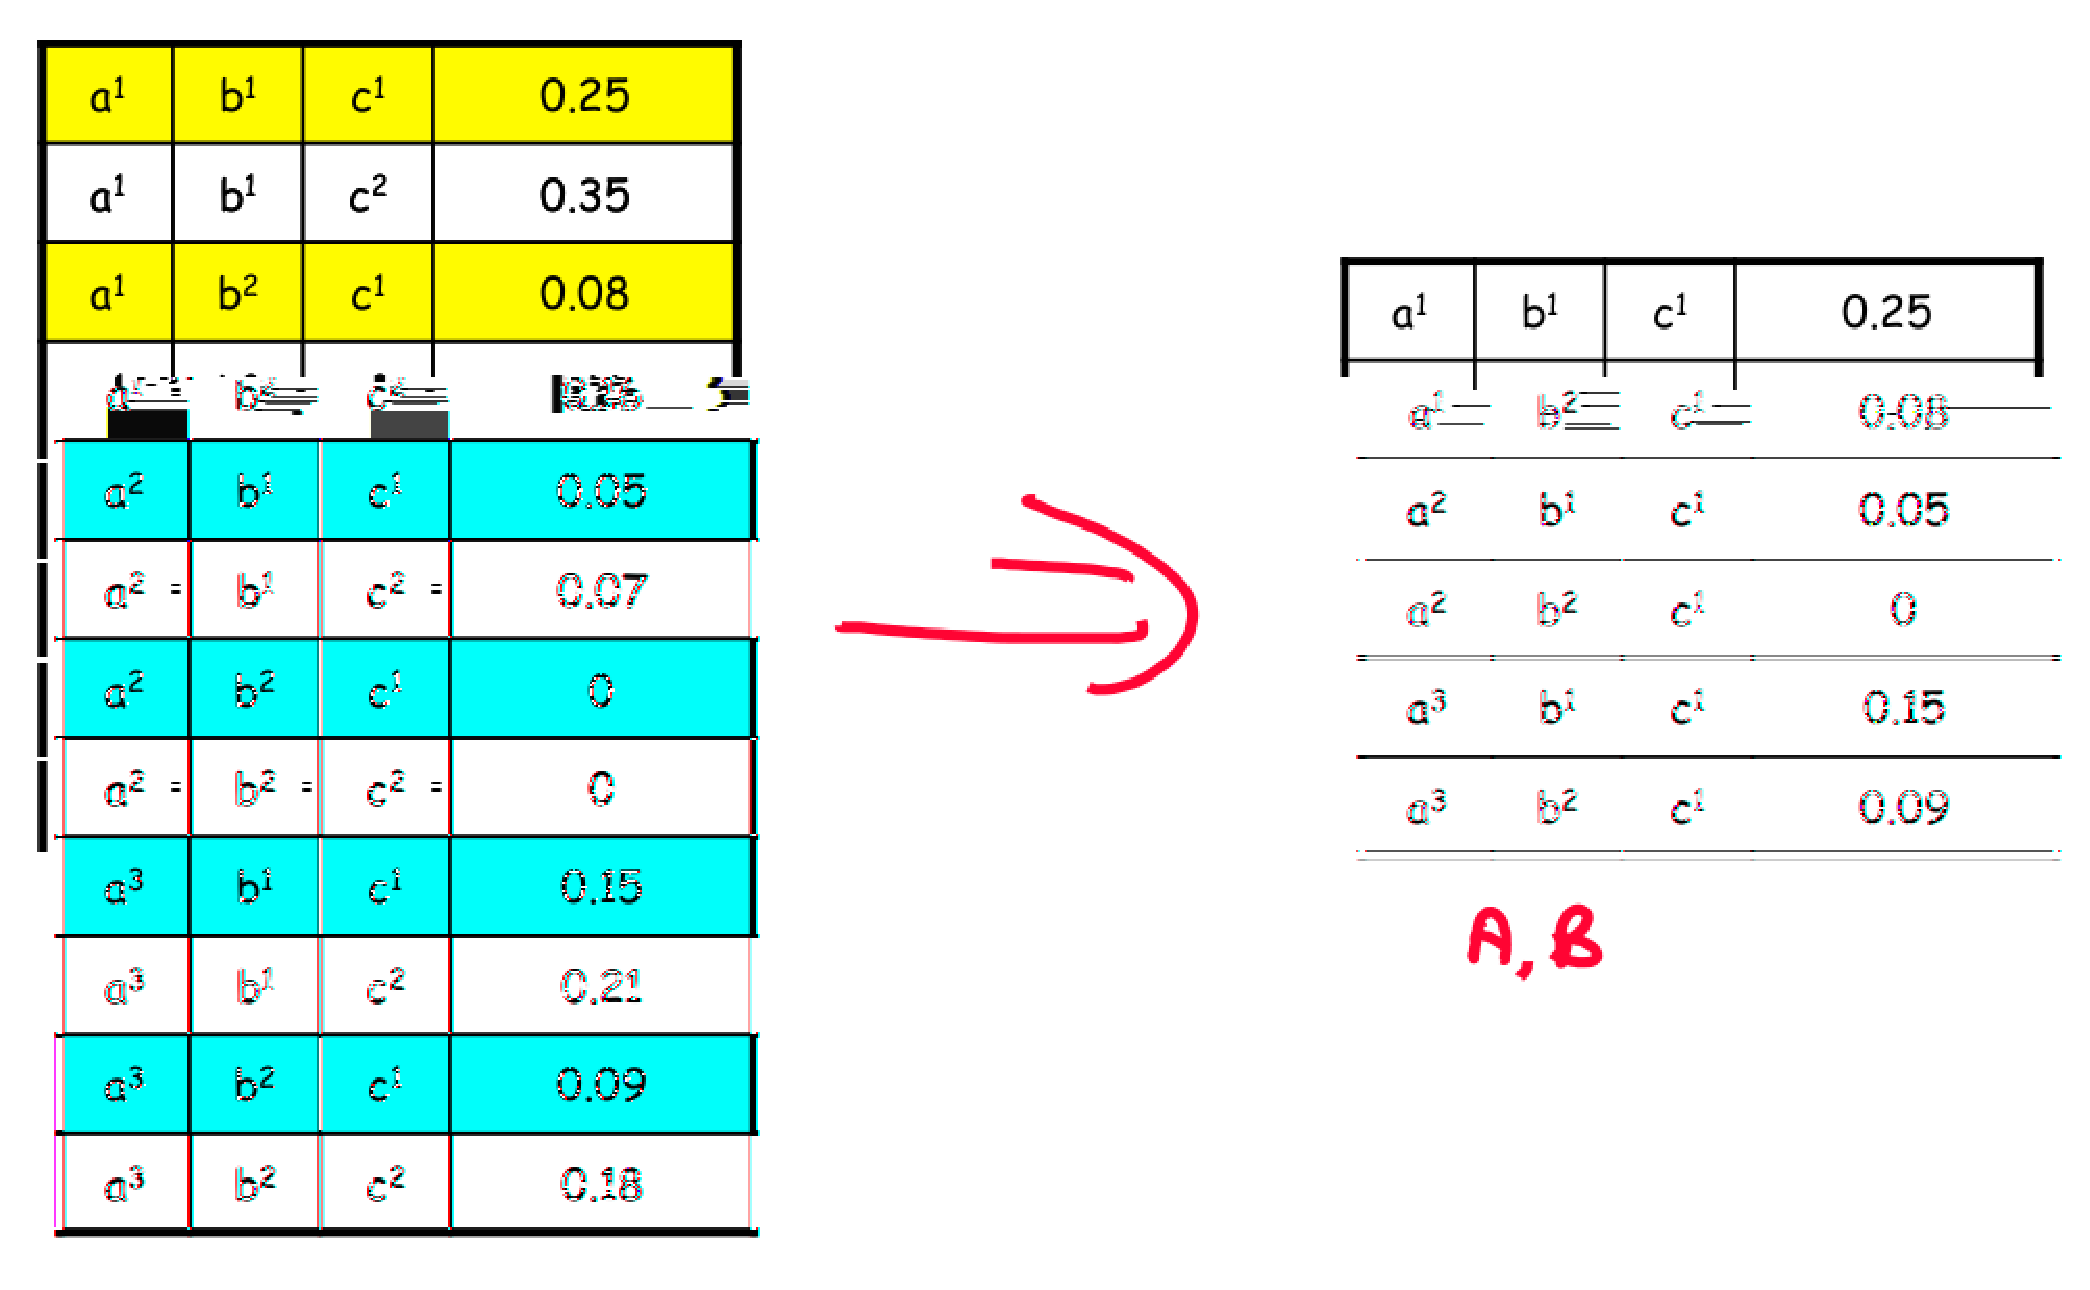
\includegraphics[scale = 0.35]{w1FactReduce}
\caption{Factor Reduction}
\label{w1FactReduce}
\end{figure}

\section{Semantics And Factorization}
\subsection{The Student Example}
The student example involving the situation where students take a course. It contains the following random variables:
\begin{itemize}
	\item Course \textbf{D}ifficulty $(D)$ ($0$ = not difficult, $1$ = difficult)
	\item Student \textbf{I}ntelligence $(I)$ ($0$ = not intelligent, $1$ = intelligent)
	\item \textbf{G}rade $(G)$ ($1$ = A, $2$ = B, $3$ = C)
	\item Student \textbf{S}AT score $(S)$ ($0$ = not good, $1$ = good)
	\item Reference \textbf{L}etter from the prof. of this course $(L)$ ($0$ = not referred, $1$ = referred)
\end{itemize}

The dependency graph is shown in figure \ref{w1graphCPD}. Intuitively, we can see the directed edge meaning a strong relation between the 2 variables. \textbf{We also annotate each node of the dependency graph to a CPD (Conditional Probability Distribution)}. \textit{NB: I do not know where this comes from, maybe we can calculate them from the data set.} 

In this example, we have 5 nodes so we will have 5 CPD as shown in figure \ref{w1graphCPD}. We have the chain rule for Bayesian Networks in this example is described in formula below.
\begin{align}
P(G|I,D)P(S|I)P(L|G)P(D)P(I) = P(D,I,G,S,L)
\end{align}
\myaligns{Chain Rule for Bayesian Networks}
Note that this formula is derived from the standard chain rule of probability and some assumption about the independence as following:
\begin{align*}
P(I,D) 		 	&= P(D) P(I|D) = P(I) P(D)\\  
P(D,I,G) 	 	&= P(I,D) P(G|I,D) \\
P(S,D,I,G)   	&= P(D,I,G) P(S|D,I,G) = P(D,I,G) P(S|I) \\
P(L,S,D,I,G) 	&= P(S,D,I,G) P(L|S,D,I,G) = P(S,D,I,G) P(L|G) \\
				&= P(I) P(D) P(G|I,D) P(S|I) P(L|G)
\end{align*}


\begin{figure}[!ht]
\centering
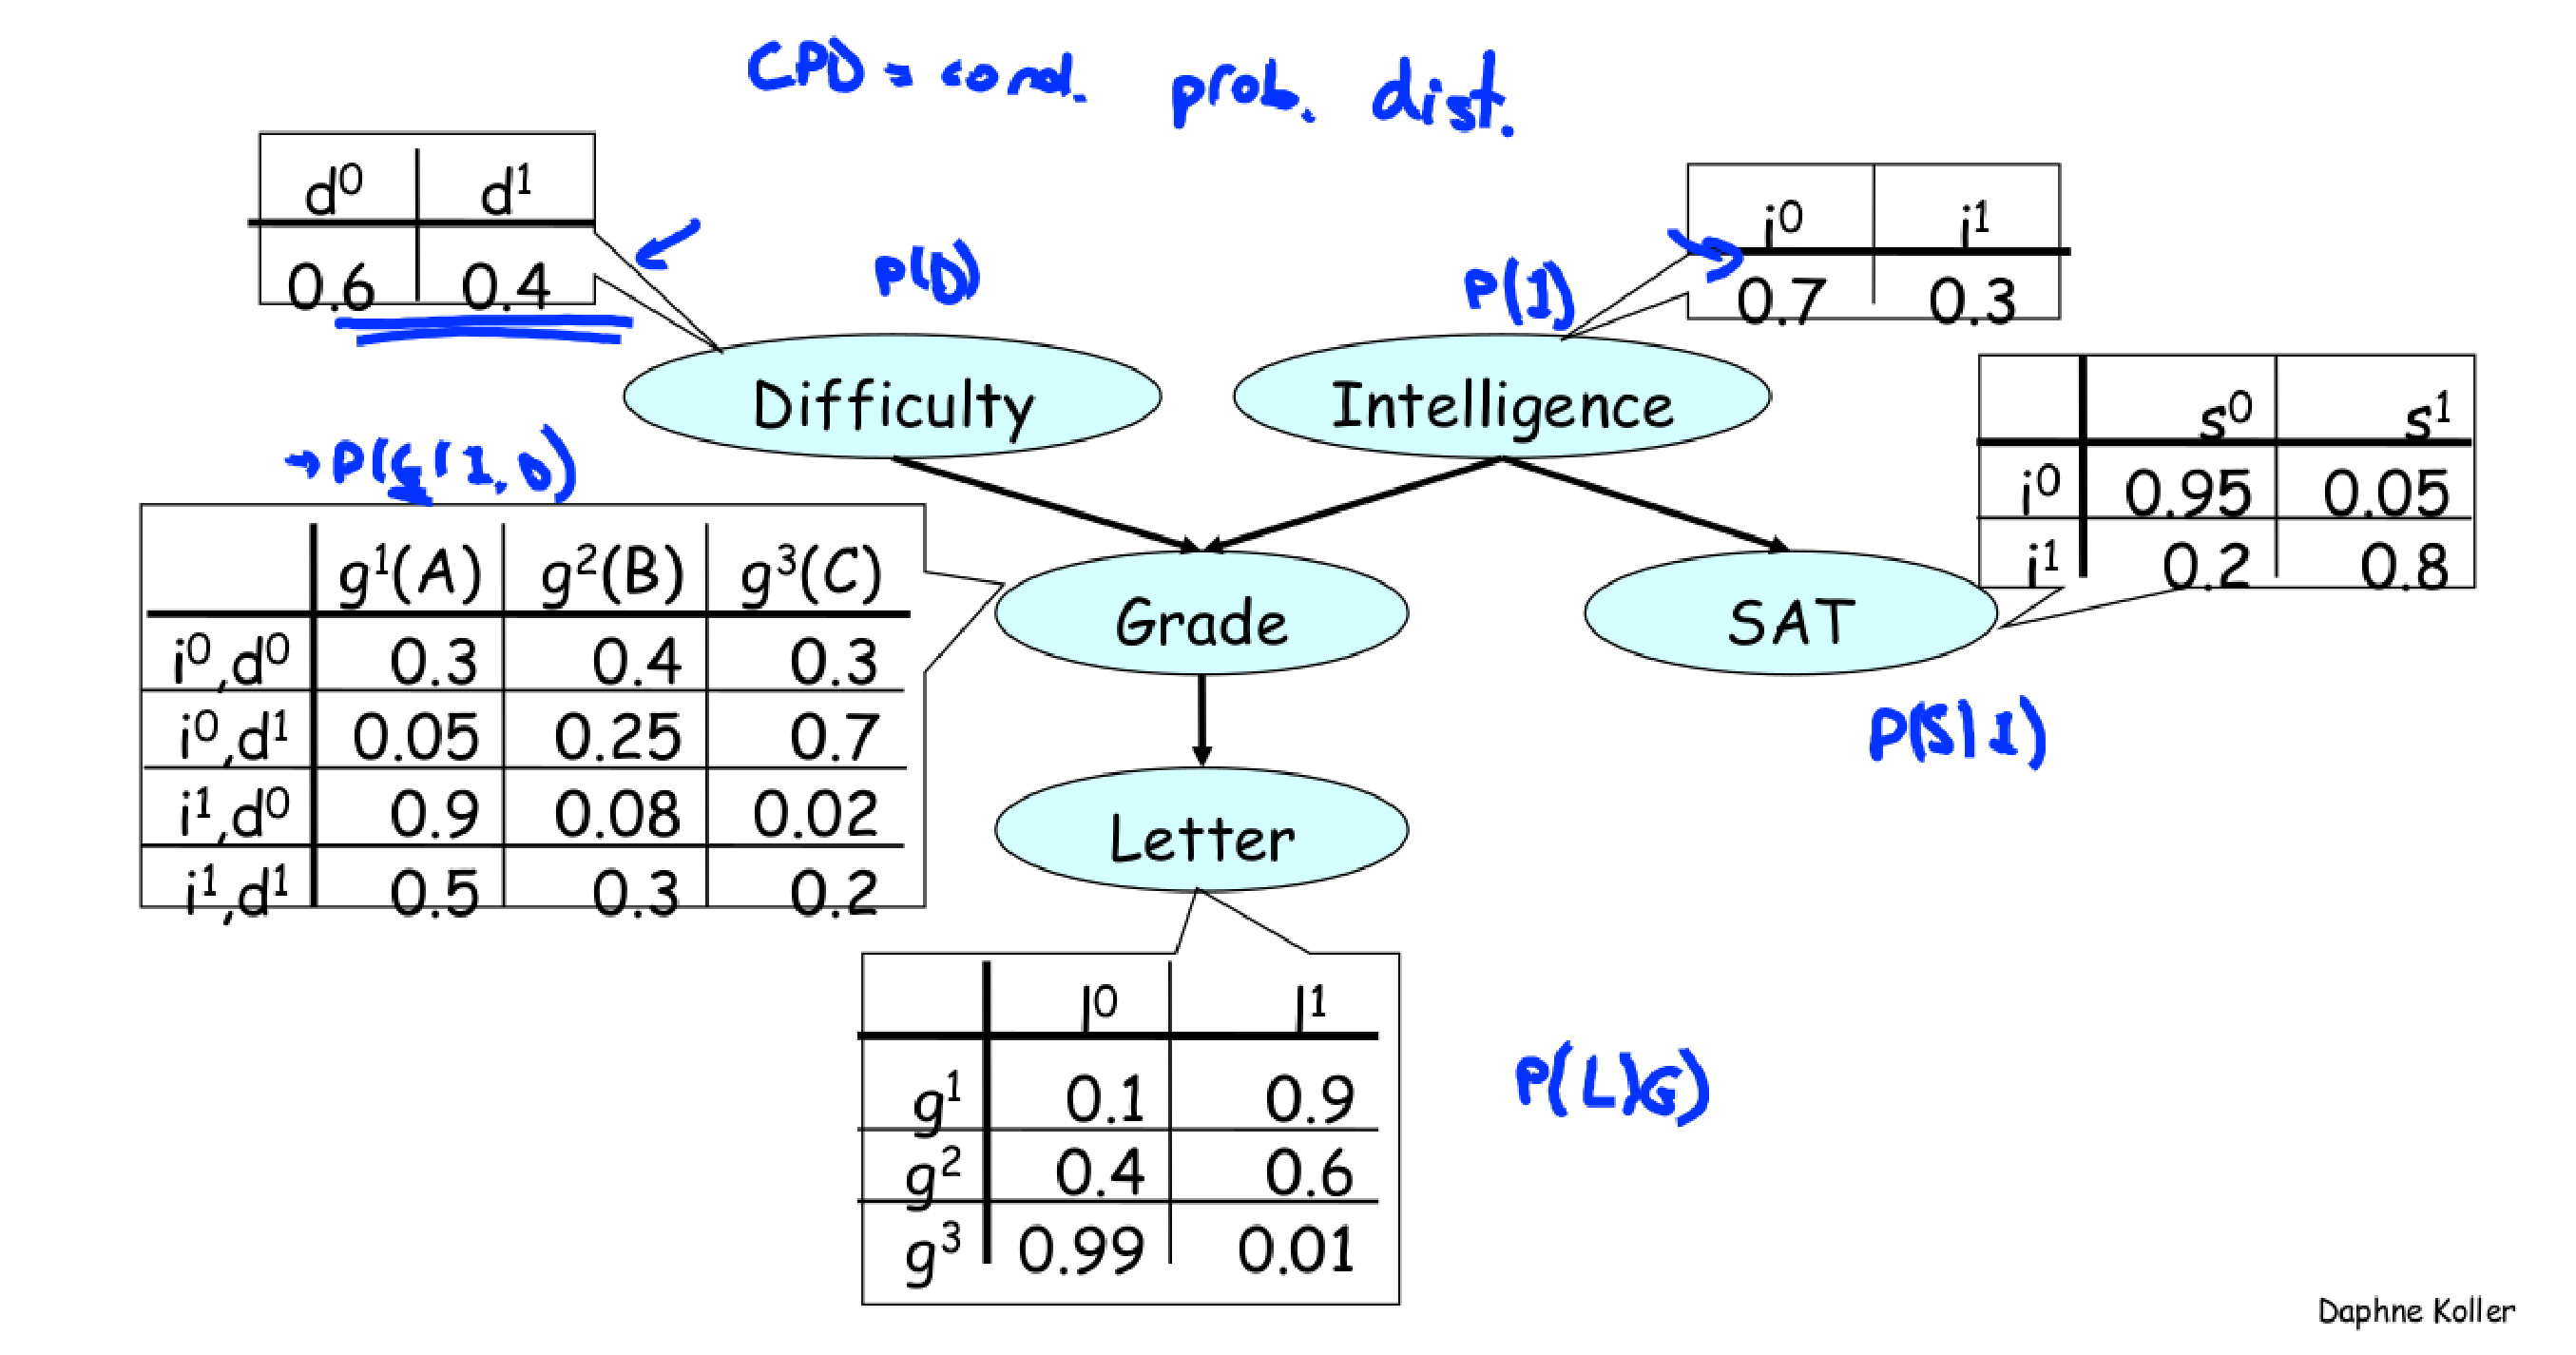
\includegraphics[scale = 0.3]{w1graphCPD}
\caption[Dependency Graph]{Dependency Graph: $D \rightarrow G$, $I \rightarrow G$, $I \rightarrow S$, $G \rightarrow L$}
\label{w1graphCPD}
\end{figure}


\subsection{Bayesian Network}
\begin{defi}[Bayesian Network]
	Bayesian Network is:
	\begin{itemize}
		\item a directed acyclic graph (DAG) G whose nodes represent the random variables $X_1,..,X_n$
		\item for each node $X_i$, there is a CPD: $P(X_i | Parents_G(X_i))$
		\item represents a joint distribution via the chain rule for Bayesian Networks in formula \ref{formChainRule} 
		\begin{align}\label{formChainRule}
		P(X_1,..,X_n) = \prod_i P(X_i|Parents_G(X_i))
		\end{align}
		\myaligns{Bayesian Network Definition}4
	\end{itemize}
\end{defi}
We can prove that Bayesian Network is a legal distribution meaning it satisfies $P \geq 0$ and $\sum_i P(X_i) = 1$. The first one is trivial. The second one is proved as follow:
\begin{align*}
\sum_{D,I,G,S,L} P(D,I,G,S,L) 	&= \sum_{D,I,G,S,L} P(D)P(I)P(G|I,D)P(S|I)P(L|G) \\
								&= \sum_{D,I,G,S} P(D)P(I)P(G|I,D)P(S|I) \sum_L P(L|G) \\
								&= \sum_{D,I,G,S} P(D)P(I)P(G|I,D)P(S|I) * 1\\
								&= \sum_{D,I,G} P(D)P(I)P(G|I,D) \sum_S P(S|I)\\
								&= \sum_{D,I} P(D)P(I) \sum_G P(G|I,D)\\
								&= ...\\
								&= 1
\end{align*}

Another notation: Let G be a graph over $X_1, .., X_n$. A distribution $P$ is called to \textbf{factorize over graph G} if:
\begin{align*}
P(X_1, .., X_n) = \prod_i P(X_i | Par_G(X_i))
\end{align*}

\section{Reasoning Patterns}

\subsection{Flow of Probabilistic Influence} \label{w1subsecFlowProbaInfl}

\subsubsection{Flow Without Evidence}
We say $X$ influence $Y$ if condition on X changes beliefs about $Y$. Hence, when we have no evidence set (observed events), $X$ can influence $Y$ when:
\begin{itemize}
	\item $X \rightarrow Y$
	\item $X \leftarrow Y$
	\item $X \rightarrow W \rightarrow Y$ 
	\item $X \leftarrow W \leftarrow Y$ 
	\item $X \leftarrow W \rightarrow Y$ 
\end{itemize}
$X$ \textbf{can not influence} $Y$ in a \textbf{v-structure}: $X \rightarrow W \leftarrow Y$. 

A trail in general is a sequence of nodes connected to each other by single edges in the graph. And an \textbf{active trail} is defined as a trail that has no v-structure in it. Such a \textbf{v-structure} is called \textbf{block} in the trail. We will redefine more formally in the next paragraph.

\subsubsection{Influence With Evidence}
Let's say we are given some evidence (observed events) $Z$. For example in figure \ref{w1graphCPD}, if we observe Intelligence, are Grade and SAT conditionally independent? 
Answer: If we don't observe Intelligence, Grade and SAT are dependent because observing Grade gives us some information about Intelligence and therefore about SAT and vice versa. However, if we observe Intelligence, then observing Grade can not affect SAT and vice versa, so they are conditionally independent.

Even when we have a evidence set $Z$, the two path $X \rightarrow Y$ and $X \leftarrow Y$ are active trail (i.e. influence can flow). Then we have 2 cases when $W \in Z$ or $W \notin Z$ shown in table \ref{w1TabFlowEvid}.

\begin{table}
\begin{tabular}{c | c | c}
Trail & $W \notin Z$ & $W \in Z$\\
\hline \hline
$X \rightarrow W \rightarrow Y$ & \textbf{Yes} & \textbf{No}  \\
\hline
$X \leftarrow W \leftarrow Y$   & \textbf{Yes} & \textbf{No}  \\
\hline
$X \leftarrow W \rightarrow Y$  & \textbf{Yes} & \textbf{No}  \\
\hline
$X \rightarrow W \leftarrow Y$  & \textbf{No}  & \textbf{Yes}  \\
								& if all of its descendants $\notin Z$ & if $W$ or one of its descendants $\in Z$ 
\end{tabular}
\caption{Influence Flow With Evidence}
\label{w1TabFlowEvid}
\end{table}

\begin{defi}[\textbf{Active Trail}]
A trail $X_1 - X_2 - ... X_k$ is \textbf{active}, given set of evidence $Z$ if:
\begin{itemize}
	\item for any v-structure $X_{i-1} \rightarrow X_i \leftarrow X_{i+1}$ we have that $X_i$ or one of its descendants $\in Z$. If so we denote that the v-structure is \textbf{activated}.
	\item $\forall X_i \notin VST \rightarrow X_i \notin Z$, where $VST$ is set of all mid nodes in v-structures of the trail.
\end{itemize}	
\end{defi}
\mydefs{Active Trail}

\subsection{Independent Parameters}
A multinomial distribution over $m$ possibilities $x_1, ..., x_m$ has $m$ parameters but only $m-1$ of them are independent because we have the constraint that all parameters must sum to 1. In a CPD $P(X|Y)$ if $X$ has $m$ values and $Y$ has $k$ values, then we have $k$ distinct multinomial distributions, one for each value of $Y$, and we have $m-1$ independent parameters in each of them, hence a total of $k(m-1)$. More generally, in a CPD $P(X|Y_1, ..., Y_r)$, if each $Y_i$ has $k_i$ values, we have a total of $k_1*...*k_r*(m-1)$ independent parameters.

Consider a simple graphical model that just had $X \rightarrow Y$ where both variables are binary. As the flow is from $X$ to $Y$, the CPD of $X$ is just $P(X)$ and $X$ is binary so the independent parameter for CPD of $X$ is 1. Now we look at $Y$: CPD of $Y$ contains 4 entries: $P(Y = 0 | X = 1)$, $P(Y = 0 | X = 0)$, $P(Y = 1 | X = 1)$, $P(Y = 1 | X = 0)$. As $P(Y = 0 | X = 1)$ and $P(Y = 1 | X = 1)$ sum to 1, and $P(Y = 0 | X = 0)$, $P(Y = 1 | X = 0)$ sum to 1, we have 2 independent parameters to define the CPD of $Y$. If we apply the formula above for $P(Y | X)$ then $r = 1$, $k_1 = 2$ as $X$ is binary, $m_Y = 2$ as $Y$ is also binary, finally we have $2*(2-1) = 2$ independent parameters.

\subsection{Inter-Causal Reasoning Example}
Figure \ref{w1InterCausualExp} shows some information about an inter-causal case. For convenience, we represent Accident by A, President by P, Traffic by T. We will calculate $P(A = 1 | T = 1)$ and $P(A = 1 | T = 1, P = 1)$. We expect that $P(A = 1 | T = 1) > P(A = 1)$ and $P(A = 1 | T = 1, P = 1) < P(A = 1 | T = 1)$.

\begin{figure}[!ht]
	\centering
	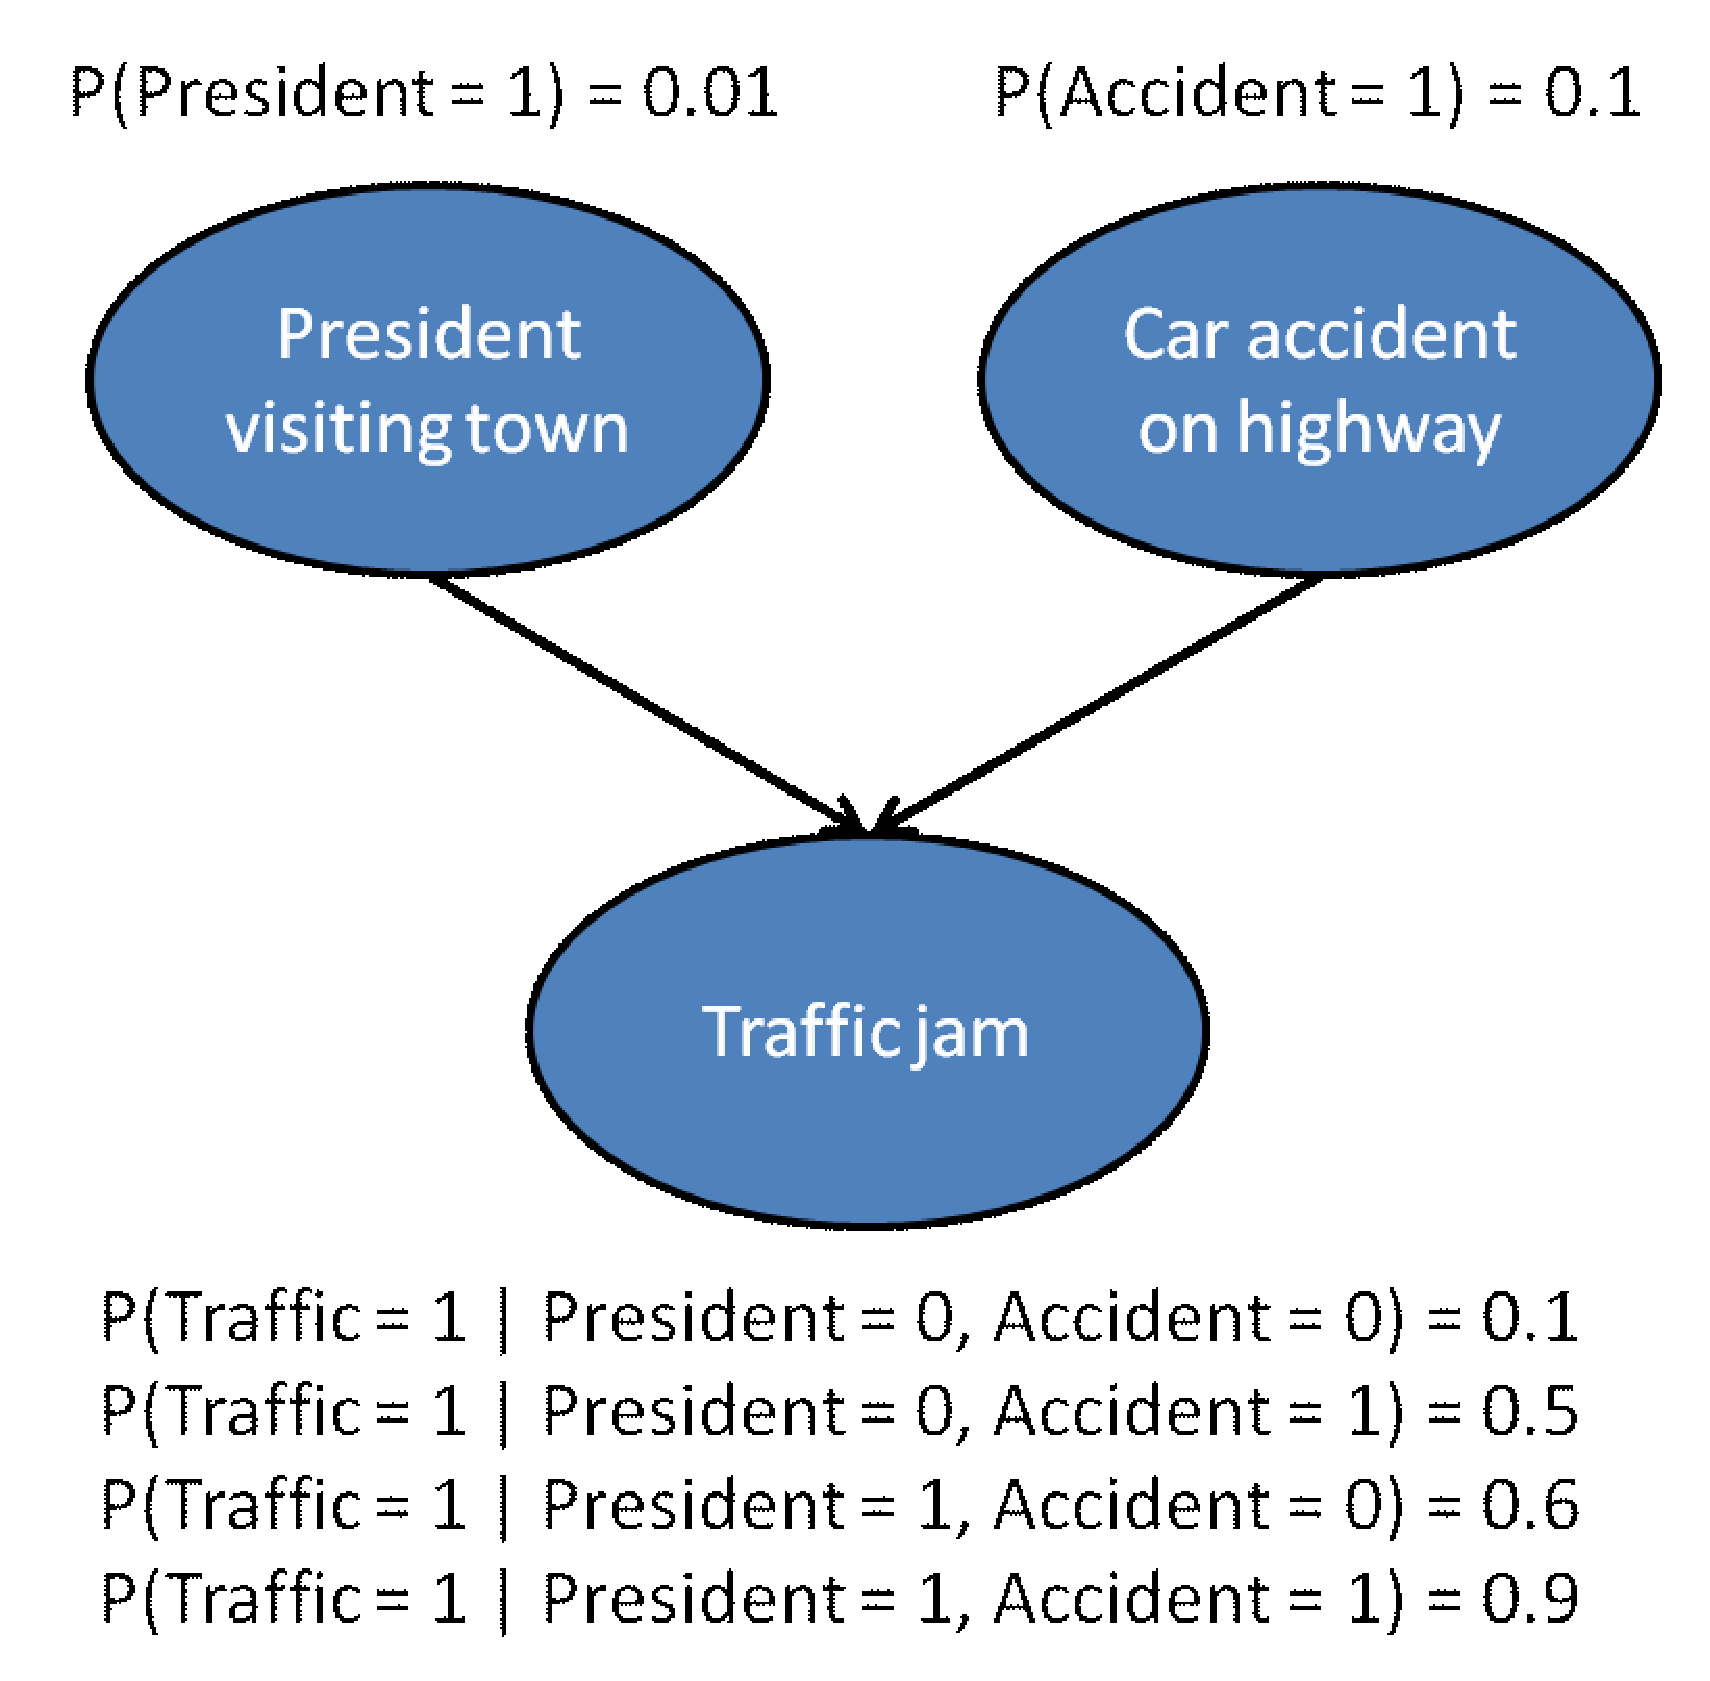
\includegraphics[scale = 0.3]{w1InterCausualExp}
	\caption{Inter-causal Reasoning Example}
	\label{w1InterCausualExp}
\end{figure}
 
Remind that the Bayes'rule is:
\begin{align*}
P(A|T) = \frac{P(A,T)}{P(T)}
\end{align*}

We need also some tricks to calculate the CPD required:

\begin{align*}
P(A, T) &= \sum_{P}P(A, T, P) = P(A, T, P=0) + P(A, T, P=1) \\
		&= P(T | A, P=0)P(A, P=0) + P(T | A, P=1)P(A, P=1) \\
		&= P(T | A, P=0)P(A)P(P=0) + P(T | A, P=1)P(A)P(P=1)
\end{align*}

And the same for $P(T)$:
\begin{align*}
P(T) 	&= \sum_{A, P}P(T, A, P) \\ 
		&= P(T, A = 0, P = 0) + P(T, A = 0, P = 1) \\ 
		& \hspace{0.5cm} + P(T, A = 1, P = 0) + P(T, A = 1, P = 1)
\end{align*}

More concretely, to compute the second CPD we apply Bayes' rule:
\begin{align} 
P(A = 1 | T = 1, P = 1) &= \frac{P(A = 1, T = 1, P = 1)}{P(T = 1, P = 1)} \\ &= \frac{P(A = 1, T = 1, P = 1)}{P(A = 0, T = 1, P = 1) + P(A = 1, T = 1, P = 1)} 
\end{align}

Then use the chain rule of Bayesian networks:
\begin{align} 
P(A = 1, T = 1, P = 1) &= P(P = 1) \times P(A = 1) \times P(T = 1 | P = 1, A = 1)
\end{align}

Applying numerical values, we obtain: $P( A = 1 | T = 1) \approx 0.35$ and $P(A = 1 | T = 1, P = 1) \approx 0.14$ this is coherent to what expected.


\subsection{Causal Reasoning}
In a Bayesian network, if there is a path from one random variable to another, then the variable at the root of the path is said to affect the other random variables in the path via causal reasoning. For example, if $A \rightarrow B \rightarrow C$, then $A$ affects $B$ and $C$ via causal reasoning and $P(C)$ is generally \textbf{not equal} to $P(C|A)$.
Intuitively, inference goes in causal direction (direction of edges): \textbf{top down}.

\subsection{Evidential Reasoning}
In a Bayesian network, if there is a path from one random variable to another, then the variable at the end of the path is said to affect the other random variables in the path via evidential reasoning. For example, if $A \rightarrow B \rightarrow C$, then $C$ affects $A$ and $B$ via evidential reasoning and $P(A)$ is generally not equal to $P(A|C)$.
Bottom up: Condition the result, ask what the probability of the initial variables was (back from the cause), using Bayes' rule.

\subsection{Inter-causal Reasoning}
Flow of information between (for example) two causes of a single effect. When you condition the result, the causes are \textbf{no longer independent}. This also works across several edges and nodes. Don't really understand "explain away"! 


\section{Conditional Independence}
For events $\alpha$, $\beta$, probability $P$ is said to satisfy $\alpha$ is independent of $\beta$ (denoted as $P \models \alpha \perp \beta$) if one of the following holds:
\begin{itemize}
	\item $P(\alpha, \beta) = P(\alpha) P(\beta)$
	\item $P(\alpha | \beta) = P(\alpha)$
	\item $P(\beta  | \alpha) = P(\beta)$
\end{itemize}

The same definition for random variables $X$ and $Y$: probability $P$ is said to satisfy $X$ is independent of $Y$ (denoted as $P \models X \perp Y$) if one of the following holds:
\begin{itemize}
	\item $P(X, Y) = P(X) P(Y)$
	\item $P(X | Y) = P(X)$
	\item $P(Y | X) = P(Y)$
\end{itemize}

Note that the second definition is a universal form of the first i.e. every events over possible values of $X$ and $Y$ must hold the first definition. We now move on to our main concept i.e. \textbf{conditional independence}. 

\begin{defi}
For (sets of) random variables $X$, $Y$, $Z$, $P$ satisfies $X$ is independent of $Y$ given $Z$ (denoted as $P \models (X \perp Y | Z)$) if one of the following holds:
\begin{itemize}
	\item $P(X,Y |Z) = P(X|Z)P(Y|Z)$
	\item $P(X   |Y,Z) = P(X|Z)$
	\item $P(Y   |X,Z) = P(Y|Z)$
	\item $P(X,Y,Z) \propto \phi_1(X,Z) \phi_2(Y,Z)$ where $\phi_1(X,Z)$ is factor over $X$ and $Z$, $\phi_2(Y,Z)$ is factor over $Y$ and $Z$.
\end{itemize}	
\end{defi}
\mydefs{Conditional Independence}

\subsection{Example}
Suppose we have 2 coins that look similar but one coin is fair and the other is biased with 90\% head. We pick a coin and toss it twice and the random variable is denoted $X_1$ and $X_2$. If we do not know which coin picked, then $X_1$ and $X_2$ are dependent of each other. For example event $X_1 = head$ will give a higher probability for $X_2 = head$. But if we know that the coin is fair or biased then $X_1$ and $X_2$ become independent (with $p = 0.5$ and $p=0.9$ respectively). 

Note that conditioning can also lose independence. Look back at the dependency graph at figure \ref{w1graphCPD}, as what we learn from subsection \ref{w1subsecFlowProbaInfl}, that $P(I, D | G)$ is not a conditional independence although $I$ and $D$ are independent. In addition, $P(S,G | I)$ is conditional independence. 

\section{Independences in Bayesian Network}
Given a graph $G$ and a distribution $P$ that \textbf{factorizes} over graph $G$. We first define \textbf{d-separation} context as follow:
\begin{defi}[d-separation]
	Node $X$ and $Y$ are \textbf{d-separated} in graph $G$ given $Z$ if there is no active trail in $G$ between $X$ and $Y$ given $Z$. Notation is: $d\text{-}sep_G(X,Y|Z)$
\end{defi}
\mydefs{d-separation}
We can intuitively see that d-separation implies independence. The formal proof is detailed in the book of Professor Koller. 
\begin{theorem}
If $P$ factorizes over $G$, and $d\text{-}sep_G(X,Y|Z)$ then $P \models (X \perp Y | Z)$.
\end{theorem}

We also have the following property:
\begin{theorem}
Any node is d-separated from its non-descendants, given its parents. Or equivalently, if $P$ factorizes $G$, then in $P$, any variable is independent of its non-descendants, given its parents.
\end{theorem}

\begin{defi}[I-maps]
	I-maps is the set of all independencies that are derived from d-separation: 
	$$ I(G) = \{(X \perp Y | Z) : d\text{-}sep_G(X,Y | Z)\} $$
	If $P$ satisfies $I(G)$ we say that $G$ is an I-map (independency map) of $P$.
\end{defi}
\mydefs{I-maps}

An example is illustrated in figure \ref{w1ImapExp}. $G_1$ is the only graph that has an independence structure which is $D \perp I$, while $G_2$ has no independence relation. Hence, both $P_1$ and $P_2$ satisfy the assumption of independence in $G_2$. We can also state that $G_2$ is an Imap of $P_1$ and $P_2$. Now look at $P_1$ and $P_2$, we can compute the marginal probability $i^0$, $i^1$, $d^0$, $d^1$ by summing over the other variable. Now we can see that under $P_1$, $I$ and $D$ are independent because $P(i^m, d_n) = P(i^m)P(d^n)$. However, under $P_2$ this does not hold. So, $G_1$ is an I-map of $P_1$ and \textbf{not} an I-map of $P_2$.

\begin{figure}[!ht]
	\centering
	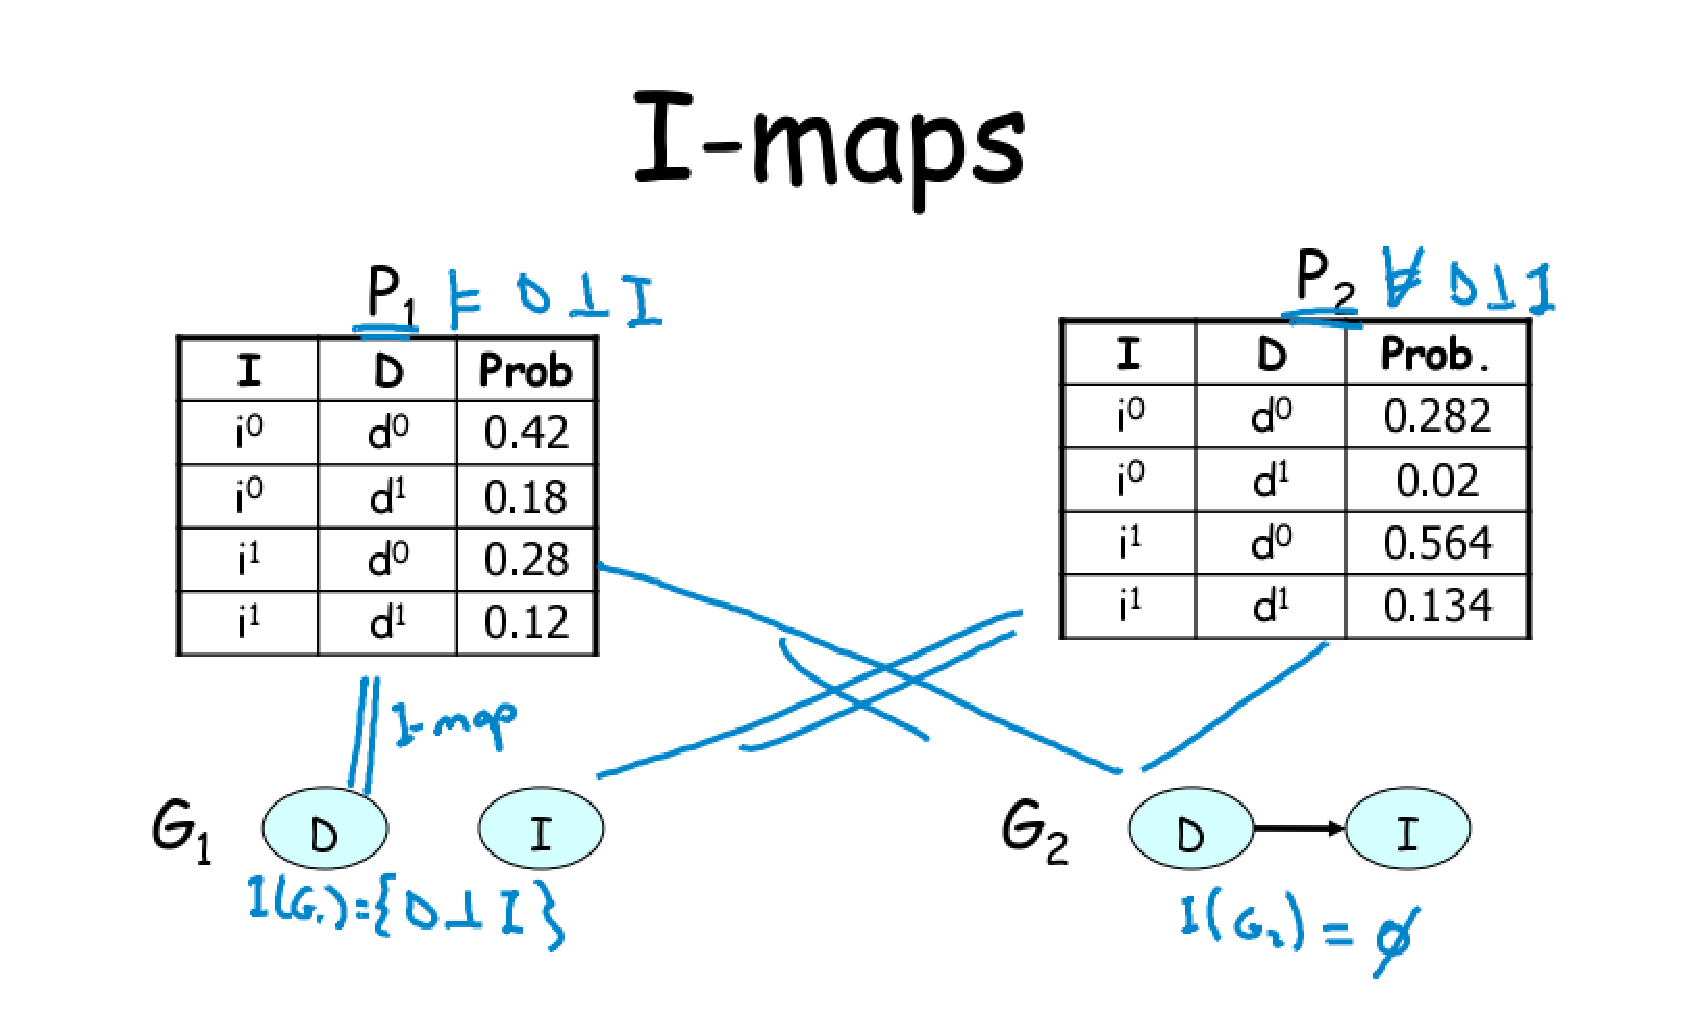
\includegraphics[scale = 0.5]{w1ImapExp}
	\caption{I-map Example}
	\label{w1ImapExp}
\end{figure}

\begin{theorem}
	If $P$ factorizes over $G$ (i.e. $P$ is representable of the bayesian network over $G$), then $G$ is an I-map for $P$. 
\end{theorem}
The above theorem means that we can read from $G$ the independencies in $P$ regardless of parameters. Interestingly, the converse of this theorem also holds:
\begin{theorem}\label{w1TheoImapFact}
	If $G$ is an I-map for $P$, then $P$ factorizes over $G$.
\end{theorem}

We can illustrate this via the Student Example in figure \ref{w1graphCPD}. Apply chain rule of probabilities:
\[ P(D,I,G,S,L) =  P(D) P(I|D) P(G|D,I)P(S|D,I,G)P(L|D,I,G,S) \]
Now from the theorem \ref{w1TheoImapFact}, if $G$ is an I-map for $P$ meaning $P$ satisfies all independencies derived from the graph meaning all the following holds:
\begin{align*}
P(I|D) &= P(I) \\
P(S|D,I,G) &= P(S|I) \\
P(L|D,I,G,S) &= P(L|G)
\end{align*} 
Apply the above expressions in the chain rule of probabilities gives us:
\[ P(D,I,G,S,L) =  P(D)P(I)P(G|D,I)P(S|I)P(L|G) \]
This is equivalent to the definition of $P$ factorizes over $G$.
